\section{提案手法の利用プロセス}
\label{sec:process}

本提案手法の利用プロセスは、以下の2ステップから構成される（図\ref{fig:process_flow}参照）。

\begin{figure}[htbp]
  \centering
  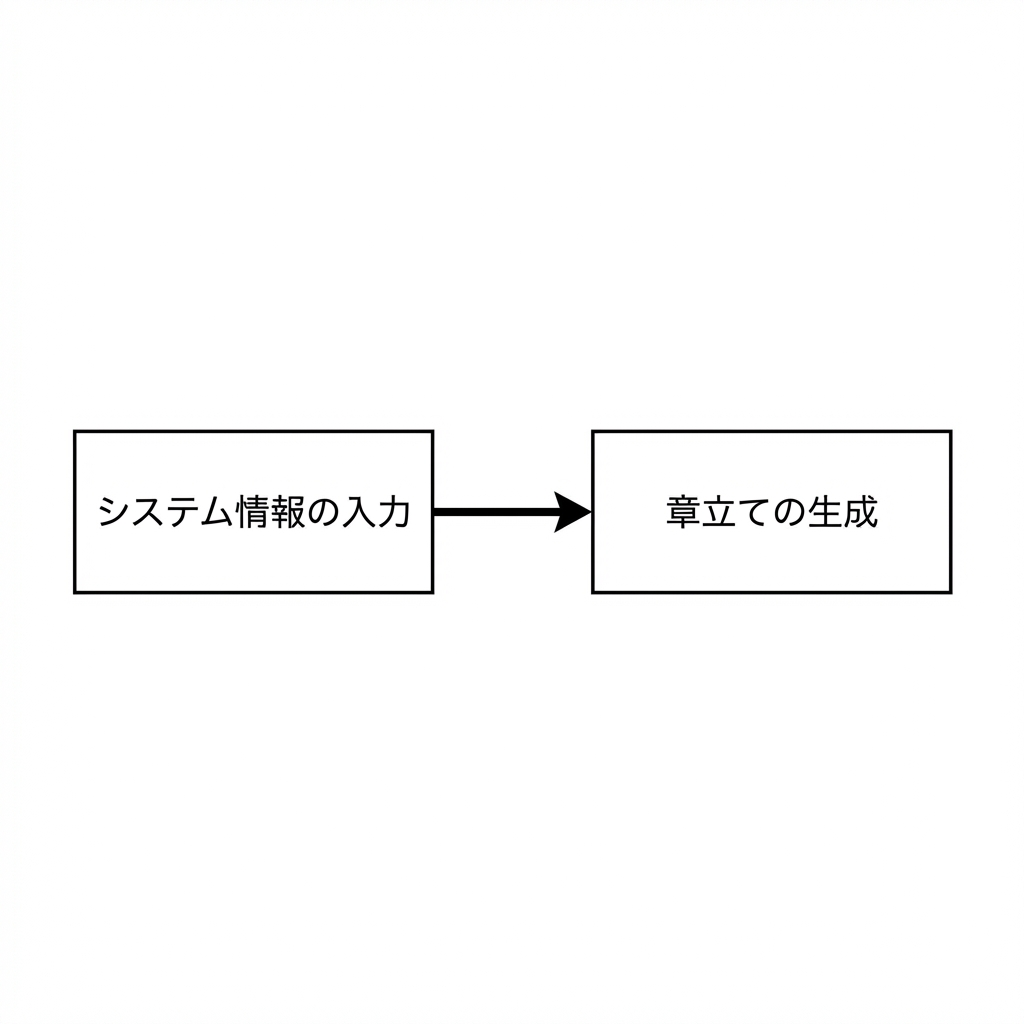
\includegraphics[width=0.8\linewidth]{./images/proposal_process_flow.png}
  \caption{提案手法によるシステム仕様書作成のフロー}
  \label{fig:process_flow}
\end{figure}

\begin{enumerate}
    \item \textbf{システム情報の入力}:
    ユーザー（開発者）は、本研究で作成したプロンプトの「開発するシステム情報」欄に、対象システムの概要を記述する。また必要に応じて「システム仕様書の定義」の微調整を行う。

    \item \textbf{章立ての生成}:
    情報を入力したプロンプトをLLMに入力し、システム仕様書の章立てを生成させる。出力結果として、章・節・項の構造と、各章に記述すべき内容の指針が得られる。
\end{enumerate}

本研究では、このプロセスによって出力された章立てが、実用的なシステム仕様書の骨子として十分に機能するかを特に重視している。
